

%% AP Physics MC Questions Archive
%%----------------------------------------


%% Second Law Inclines
%%----------------------------------------
\element{ap}{
\begin{question}{second-law-inclines-q01}
    Base your answer to the following question on the picture below which shows a \SI{3}{\kilo\gram} block sliding \SI{50}{\meter} down a frictionless inclined plane dropping a distance of 30 m.
    \begin{center}
    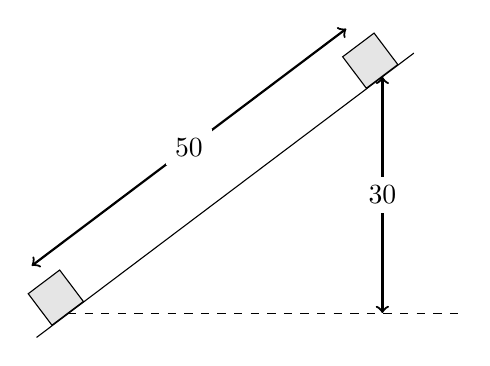
\begin{tikzpicture}
        %% Plane
        \draw (0,0) -- (37:6);
        %% Blocks
        \node[draw,rotate=37,anchor=south,minimum size=0.5cm,fill=white!90!black] (A) at (37:0.5) {};
        \node[draw,rotate=37,anchor=south,minimum size=0.5cm,fill=white!90!black] (B) at (37:5.5) {};
        %% Lables
        \draw[<->,thick] (A.north) ++(127:0.25) -- ++(37:5) node[pos=0.5,anchor=center,fill=white] {\SI{50}{\meter}};
        \draw[<->,thick] (37:5.5) --++(270:3) node[fill=white,pos=0.5,anchor=center] {\SI{30}{\meter}};
        \draw[dashed] (37:0.5) -- ++(0:5);
    \end{tikzpicture}
    \end{center}
    What is the magnitude of the acceleration for the block?
    \begin{multicols}{3}
    \begin{choices}
        \wrongchoice{\SI{3}{\meter\per\second\squared}}
        \wrongchoice{\SI{4}{\meter\per\second\squared}}
      \correctchoice{\SI{6}{\meter\per\second\squared}}
        \wrongchoice{\SI{8}{\meter\per\second\squared}}
        \wrongchoice{\SI{10}{\meter\per\second\squared}}
    \end{choices}
    \end{multicols}
\end{question}
}

\element{ap}{
\begin{question}{second-law-inclines-q02}
    Base your answer to the following question on the picture below,
        which represents a plane \SI{10}{\meter} in length with a coefficient of kinetic friction of \num{0.2},
        inclined at an angle of \ang{53}.
    A block of weight \SI{30}{\newton} is placed at the top of the plane and allowed to slide down.
    \begin{center}
    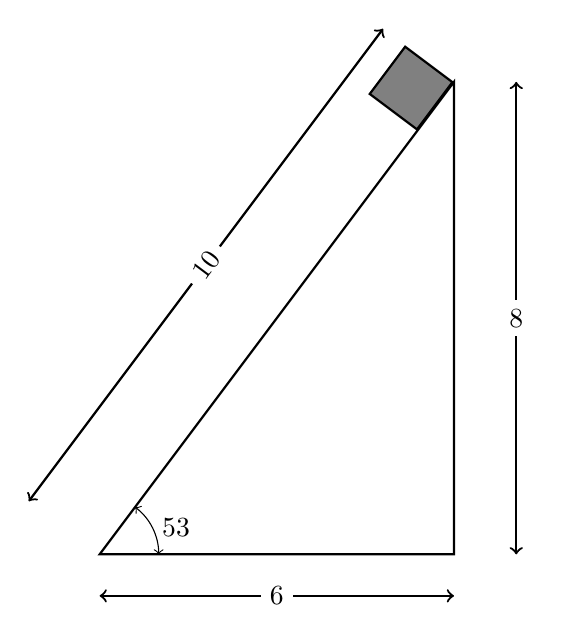
\begin{tikzpicture}[scale=0.75]
        %% Triangle
        \draw[thick] (0,0) -- (6,0) -- (6,8) -- cycle;
        %% Labels
        \draw[<->] (1,0) arc (0:53.13:1) node[pos=0.5,anchor=west] {\ang{53}};
        \draw[<->,thick] (0,-2em) -- (6,-2em) node[pos=0.5,anchor=center,fill=white] {\SI{6}{\meter}};
        \draw[<->,thick] (6cm+3em,0) -- (6cm+3em,8) node[pos=0.5,anchor=center,fill=white] {\SI{8}{\meter}};
        \draw[<->,thick] (143.13:1.5) -- ++(53.13:10) node[pos=0.5,anchor=center,rotate=53.13,fill=white] {\SI{10}{\meter}};
        %% block
        \node[draw,thick,minimum size=0.75cm,fill=white!50!black,rotate=53.13,anchor=south east] (A) at (53.13:10cm) {};
    \end{tikzpicture}
    \end{center}
    The magnitude of the normal force exerted on the block by the plane is most nearly:
    \begin{multicols}{3}
    \begin{choices}
        \wrongchoice{\SI{15}{\newton}}
      \correctchoice{\SI{18}{\newton}}
        \wrongchoice{\SI{24}{\newton}}
        \wrongchoice{\SI{30}{\newton}}
        \wrongchoice{\SI{50}{\newton}}
    \end{choices}
    \end{multicols}
\end{question}
}

\newcommand{\apSecondLawInclinesQThree}{
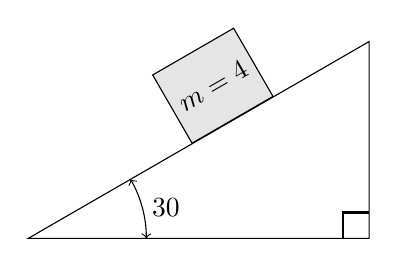
\begin{tikzpicture}
    %% Floor and plane
    \draw (0,0) -- (4.33,2.5) -- (4.33,0) -- cycle;
    \draw[thick] (4,0) -- (4,0.33) -- (4.33,0.33);
    %% angle
    \draw[<->] (1.5,0) arc(0:30:1.5) node[pos=0.5,anchor=west] {\ang{30}};
    %% block
    \node[draw,minimum size=1cm,anchor=south,rotate=30,fill=white!90!black] at (30:3) {$m=\SI{4}{\kilo\gram}$};
\end{tikzpicture}
}

\element{ap}{
\begin{question}{second-law-inclines-q03}
    %Base your answers to questions 3 through 5 on the following diagram,
    %    which shows a block sliding down a frictionless ramp.
    The diagram below shows a block sliding down a frictionless ramp.
    The block starts at the top of the ramp and takes \SI{4}{\second} to slide to the bottom of the ramp.
    \begin{center}
        \apSecondLawInclinesQThree
    \end{center}
    How high is the top of the ramp?
    \begin{multicols}{3}
    \begin{choices}
        \wrongchoice{\SI{5}{\meter}}
        \wrongchoice{\SI{10}{\meter}}
      \correctchoice{\SI{20}{\meter}}
        \wrongchoice{\SI{25}{\meter}}
        \wrongchoice{\SI{40}{\meter}}
    \end{choices}
    \end{multicols}
\end{question}
}

\element{ap}{
\begin{question}{second-law-inclines-q04}
    %Base your answers to questions 3 through 5 on the following diagram,
    %    which shows a block sliding down a frictionless ramp.
    The diagram below shows a block sliding down a frictionless ramp.
    The block starts at the top of the ramp and takes \SI{4}{\second} to slide to the bottom of the ramp.
    \begin{center}
        \apSecondLawInclinesQThree
    \end{center}
    The speed of the block when it reaches the bottom of the ramp is most nearly:
    \begin{multicols}{3}
    \begin{choices}
        \wrongchoice{\SI{4}{\meter\per\second}}
        \wrongchoice{\SI{8}{\meter\per\second}}
        \wrongchoice{\SI{14}{\meter\per\second}}
      \correctchoice{\SI{20}{\meter\per\second}}
        \wrongchoice{\SI{40}{\meter\per\second}}
    \end{choices}
    \end{multicols}
\end{question}
}

\element{ap}{
\begin{question}{second-law-inclines-q05}
    %Base your answers to questions 3 through 5 on the following diagram,
    %    which shows a block sliding down a frictionless ramp.
    The diagram below shows a block sliding down a frictionless ramp.
    The block starts at the top of the ramp and takes \SI{4}{\second} to slide to the bottom of the ramp.
    \begin{center}
        \apSecondLawInclinesQThree
    \end{center}
    If the coefficient of kinetic friction between the block and the incline is \num{0.4},
        the work that the normal force does on the block during the slide is:
    %% NOTE: TODO: double check this
    %% did they mean to say normal force or friction
    \begin{multicols}{3}
    \begin{choices}
        \wrongchoice{zero}
        \wrongchoice{\SI{20}{\joule}}
        \wrongchoice{\SI{240}{\joule}}
      \correctchoice{\SI{550}{\joule}}
        \wrongchoice{\SI{700}{\joule}}
    \end{choices}
    \end{multicols}
\end{question}
}

\newcommand{\apSecondLawInclinesQSix}{
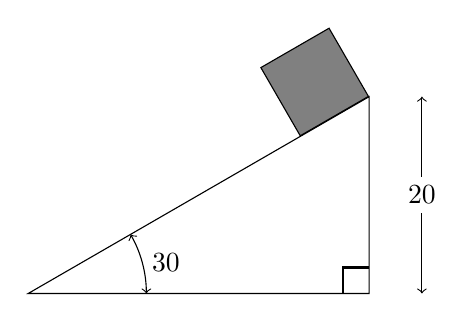
\begin{tikzpicture}
    %% Floor and plane
    \draw (0,0) -- (4.33,2.5) -- (4.33,0) -- cycle;
    \draw[thick] (4,0) -- (4,0.33) -- (4.33,0.33);
    %% angle
    \draw[<->] (1.5,0) arc(0:30:1.5) node[pos=0.5,anchor=west] {\ang{30}};
    %% block
    \node[draw,minimum size=1cm,anchor=south east,rotate=30,fill=white!50!black] at (30:5) {};
    %% distance
    \draw[<->] (5,0) -- (5,2.5) node[pos=0.5,anchor=center,fill=white] {\SI{20}{\meter}};
\end{tikzpicture}
}

\element{ap}{
\begin{question}{second-law-inclines-q06}
    %Base your answers to questions 6 through 8 on the following diagram,
    Base your answers on the following diagram,
        which shows a block that starts at the top of a frictionless ramp and slides down.
    \begin{center}
        \apSecondLawInclinesQSix
    \end{center}
    How long does it take to block to slide to the bottom of the ramp?
    \begin{multicols}{2}
    \begin{choices}
      \correctchoice{\SI{4}{\second}}
        \wrongchoice{\SI{8}{\second}}
        \wrongchoice{\SI{10}{\second}}
        \wrongchoice{\SI{16}{\second}}
        \wrongchoice{There is insufficient information to answer the question.}
    \end{choices}
    \end{multicols}
\end{question}
}

\element{ap}{
\begin{question}{second-law-inclines-q07}
    %Base your answers to questions 6 through 8 on the following diagram,
    Base your answers on the following diagram,
        which shows a block that starts at the top of a frictionless ramp and slides down.
    \begin{center}
        \apSecondLawInclinesQSix
    \end{center}
    With what speed will the block reach the bottom if it was released from rest at the top?
    \begin{multicols}{3}
    \begin{choices}
        \wrongchoice{\SI{10}{\meter\per\second}}
      \correctchoice{\SI{20}{\meter\per\second}}
        \wrongchoice{\SI{25}{\meter\per\second}}
        \wrongchoice{\SI{30}{\meter\per\second}}
        \wrongchoice{\SI{40}{\meter\per\second}}
    \end{choices}
    \end{multicols}
\end{question}
}

\element{ap}{
\begin{question}{second-law-inclines-q08}
    %Base your answers to questions 6 through 8 on the following diagram,
    Base your answers on the following diagram,
        which shows a block that starts at the top of a frictionless ramp and slides down.
    \begin{center}
        \apSecondLawInclinesQSix
    \end{center}
    If the mass of the block is \SI{5}{\kilo\gram},
        how much work is done by gravity as the block slides down the full length of the incline?
    \begin{multicols}{3}
    \begin{choices}
        \wrongchoice{\SI{10}{\joule}}
        \wrongchoice{\SI{100}{\joule}}
        \wrongchoice{\SI{200}{\joule}}
      \correctchoice{\SI{1000}{\joule}}
        \wrongchoice{\SI{2000}{\joule}}
    \end{choices}
    \end{multicols}
\end{question}
}

\element{ap}{
\begin{question}{second-law-inclines-q09}
    A greased pig starts at rest from the top of a frictionless slide a height \SI{25}{\meter} above his mud pit.
    If the bottom section of the slide is \SI{5}{\meter} above the pit and is parallel to the ground,
        at what distance from the bottom of the slide will the pig hit the mud?
    \begin{multicols}{3}
    \begin{choices}
        \wrongchoice{\SI{10}{\meter}}
        \wrongchoice{\SI{15}{\meter}}
      \correctchoice{\SI{20}{\meter}}
        \wrongchoice{\SI{28}{\meter}}
        \wrongchoice{\SI{36}{\meter}}
    \end{choices}
    \end{multicols}
\end{question}
}


\endinput


